%1
\part{Statistische Verfahren der Meta-Analyse}\label{part:datenanalyse}

\frame{\partpage}

\frame[allowframebreaks]{\frametitle{Statistische Verfahren der Meta-Analyse}
  \begin{footnotesize}\tableofcontents[part=4, hideallsubsections]\end{footnotesize}}

\begin{frame}
  \frametitle{Meta-Analyse auf einen Blick}
  \begin{enumerate}
  \item \emph{Ein} Ziel einer Meta-Analyse ist das Zusammenfassen einer
    Effektstärkenverteilung (ESV) mit Hilfe einer (gewichteten) mittleren ES.
  \item Die Wahl des Schätzverfahrens hängt u.a. vom Ausmaß der Unterschiede
    (Heterogenität, siehe ausführlich \pageref{fr:heterodef}) zwischen
    den ES ab. Es werden (im univariaten Fall) zwei ES-Modelle unterschieden:
    (1) Fixed-effects model (geringe Unterschiede), (2) Random-effects model
    (große Unterschiede).
  \item Neben der Bestimmung eines Mittelwertes geht es in MA \emph{auch/vor
      allem} um die Darstellung/Erfassung und Aufklärung der ES-Heterogenität
    (Regressionsmodelle oder ANOVA-ähnliche Modelle).
  \end{enumerate}
\end{frame}



\section{Befundsynthese von Aggregatdaten}


\begin{frame}
  \frametitle{Befundsynthese} Die Befundsynthese von Aggregatdaten ist ein
  typischer Anwendungsfall einer Meta-Analyse. Dabei sind die folgenden drei
  Bedingungen zu beachten:
  %
  \begin{enumerate}
  \item Die Bildung eines synthetischen Befundes ist nur sinnvoll, wenn
    mindestens zwei einzelne Statistiken berichtet werden,
  \item diese müssen i.A. statistisch unabhängig\footnote{Für abhängige Effektstärken
      gibt es spezielle Verfahren, siehe Folie \pageref{slide:abhaeng-es}.} sein und
  \item in die Mittelwertbildung gehen die einzelnen Befunde nach dem Kriterium
    ihrer Reliabilität (Fehlervarianz/quadrierter SE; Fallzahl) gewichtet ein.
  \end{enumerate}
\end{frame}



\begin{frame}
  \frametitle{Effektstärkenverteilungen beschreiben}
  \begin{itemize}
  \item Ziel ist es, den Lageparameter ("`Mittelwert"') einer ES-Verteilung zu schätzen.
  \item Schätzung ist mit stat. Unsicherheit verbunden, u.a. sind Informationen der
    SEs der einzelnen Effektstärken zu berücksichtigen.
  \item Möglicherweise aber ist die ES-Verteilung durch (unbekannte) Faktoren wie Alter
    oder Geschlecht beeinflusst, d.h. überzufällige Unterschiede zwischen
    Effektstärkengruppen.
  \item Diese Heterogenität/Zwischenstudienvariation beeinflusst die Schätzung
    des Mittelwertes und der stat. Unsicherheit.
  \item Eine zentrale Frage: Ist die ES-Heterogenität so groß, dass wir sie
    berücksichtigen müssen?
    \begin{itemize}
    \item Nein: Fixed-effects model
    \item Ja: Random-effects model
    \end{itemize}
  \end{itemize}
\end{frame}






\subsection{Fixed-effects model (FEM)}

\begin{frame}
  \frametitle{Das \emph{fixed-effects model} (FEM)}
  %%
  \begin{itemize}
  \item Annahmen
    \begin{itemize}
    \item Es gibt \emph{einen} gemeinsamen (\emph{common effect})
      Populationsparameter ($\theta$).
    \item Alle Studien sind sich sehr ähnlich (Design, Stichprobe, Operationalisierung, \ldots).
    \item Es gibt statische Belege für die Homogenität der Effektstärken (Test
      auf Heterogenität), d.h. es gibt keine (kaum) unbeobachtete Heterogenität.
    \item Man kan sich sicher sein, die allermeisten Publikationen entdeckt zu
      haben.
    \end{itemize}
  \item Konsequenzen
    \begin{itemize}
    \item Der Populationsparameter kann relativ genau geschätzt werden (kleiner
      Standardfehler, enges Konfidenzintervall).
    \item Studien mit großen Fallzahlen werden stark gewichtet.
    \end{itemize}
  \end{itemize}
\end{frame}



\begin{frame}
  \frametitle{Verteilung der wahren Effekte im FEM}
  \includegraphics[width=\textwidth]{Borenstein1}
  \newline
  Legende:
  \begin{itemize}
  \item[\FilledSmallCircle] Wahre Effektstärke in Studie $j$
  \item[\FilledSmallTriangleDown] Wahre Effektstärke über alle Studien
    (combined) ($\theta_1 = \theta_2 = \ldots = \theta$)
  \end{itemize}
  \citep[Quelle: ][64]{borenstein_introduction_2009}
\end{frame}


\begin{frame}[shrink = 5]
  \frametitle{Fehler im FEM}
  \includegraphics[width=\textwidth]{Borenstein2}
  \newline
  %%Legende: \FilledSmallCircle, \FilledSmallSquare, \FilledSmallTriangleDown, \FilledSmallDiamondshape
  Legende:
  \begin{itemize}
  \item[\FilledSmallCircle] Wahre Effektstärke in Studie $j$
  \item[\FilledSmallTriangleDown] Wahre Effektstärke über alle Studien
    (combined) ($\theta_1 = \theta_2 = \ldots = \theta$)
  \item[\FilledSmallSquare] Empirische/Beobachtete Effektstärken
  \end{itemize}
  \citep[Quelle: ][64]{borenstein_introduction_2009}
\end{frame}


\begin{frame}[shrink = 5]
  \frametitle{Befundsynthese von Aggregatdaten (FEM)}
  %%
  Gegeben seien $k$ unabhängige Effektstärken $T_j$ ($j = 1, \ldots,k$), dann
  berechnet sich die gewichtete mittlere Effektstärke nach:
  \begin{equation}
    \overline{T}_{FEM} = \frac{\sum\limits^k_{j=1}{w_j \times T_j}}{\sum\limits^k_{j=1}{w_j}},
  \end{equation}
  mit einem Gewicht $w_j$, das der inversen Fehlervarianz ($1/v_j$) bzw. dem
  inversen quadrierten Standardfehler ($1/SE_j$) der $j$-ten Effektstärke
  entspricht:
  \begin{equation}
    w_j=\frac{1}{SE^2_j} = \frac{1}{v_j}.
  \end{equation}
  Die zusammengefasste Fehlervarianz $\overline{v}_{FEM}$ selbst ergibt sich
  aus:
  \begin{equation}
    \overline{v}_{FEM}=\frac{1}{\sum\limits^k_{j=1}(1/v_j)}.
  \end{equation}
  Für den Standardfehler von $\overline{T}_{FEM}$ gilt dann $\overline{SE}_{FEM}
  = \sqrt{\overline{v}_{FEM}}$.
\end{frame}



\subsection{Random-effects model (REM)}

\begin{frame}[shrink=10]
  \frametitle{Das \emph{random-effects model} (REM)}
  %%
  \begin{itemize}
  \item Annahmen
    \begin{itemize}
    \item Jede Studie $j$ besitzt ihren eigenen Populationsparameter
      ($\theta_j$), geschätzt wird ein "`mittlerer"' Effekt (\emph{average effect}).
    \item Man kann nicht annehmen, dass alle Studien ähnlich sind (Design,
      Stichprobe, Operationalisierung, \ldots).
    \item Es lassen sich u.U. aus der Theorie Einflussgrößen ableiten, die für
      Unterschiede in den Studienbefunden verantwortlich gemacht werden können.
    \item Es gibt statische Belege für die Heterogenität der Effektstärken (Test
      auf Heterogenität).
    \item Man kan sich nicht sicher sein, die allermeisten Publikationen
      entdeckt zu haben.
    \end{itemize}
  \item Konsequenzen
    \begin{itemize}
    \item Der gemeinsame Populationsparameter kann nur ungenau geschätzt werden
      (großer Standardfehler, breites Konfidenzintervall).
    \item Die Studiengewichte werden ähnlicher, d.h. große Studien erhalten
      weniger Einfluss, kleine Studien gewinnen Einfluss.
    \end{itemize}
  \end{itemize}
\end{frame}


\begin{frame}
  \frametitle{Verteilung der wahren Effektstärken im REM}
  \includegraphics[width=\textwidth]{Borenstein5}
  \newline
  Legende:
  \begin{itemize}
  \item[\FilledSmallCircle] Wahre Effektstärke in Studie $j$
  \item[\FilledSmallTriangleDown] Mittlere ("`average"') Effektstärke über alle
    Studien (combined)
  \end{itemize}
  \citep[Quelle: ][70]{borenstein_introduction_2009}
\end{frame}


\begin{frame}[shrink = 5]
  \frametitle{Fehler im REM}
  \includegraphics[width=\textwidth]{Borenstein6}
  \newline
  %%Legende: \FilledSmallCircle, \FilledSmallSquare, \FilledSmallTriangleDown, \FilledSmallDiamondshape
  Legende:
  \begin{itemize}
  \item[\FilledSmallCircle] Wahre Effektstärke in Studie $j$
  \item[\FilledSmallSquare] Empirische/Beobachtete Effektstärken
  \item[\FilledSmallTriangleDown] Wahre Effektstärke über alle Studien (combined)
  \item Übersetzung der unterschiedlichen Nomenklatur (siehe Folie \pageref{slide:fem-refm-fehler}): $\zeta_3 = u_3$
  \end{itemize}
  \citep[Quelle: ][71]{borenstein_introduction_2009}
\end{frame}


\begin{frame}[shrink = 5]
  \frametitle{Verteilung der Stichprobenfehler im REM: Binnen- und Zwischenstudienvarianz}
  \includegraphics[width=\textwidth]{Borenstein7}
  \newline
  %%Legende: \FilledSmallCircle, \FilledSmallSquare, \FilledSmallTriangleDown, \FilledSmallDiamondshape
  Legende:
  \begin{itemize}
  \item[\FilledSmallCircle] Wahre Effektstärke in Studie $j$
  \item[\FilledSmallSquare] Empirische/Beobachtete Effektstärken (Hinweis: Studie 1 kleines N, Studie 2 großes N)
  \item[\FilledSmallTriangleDown] Mittlere ("`average"') Effektstärke über alle Studien (combined)
  \end{itemize}
  \citep[Quelle: ][71]{borenstein_introduction_2009}
\end{frame}


\begin{frame}[plain]
  \frametitle{Das REM als ein zweistufiger Prozess}
  \includegraphics[width=0.71\textwidth, angle=90]{f_rem_diagram2}


\citep[Quelle: ][]{thompson_introduction_2013, viechtbauer_accounting_2007}

%(Source: Thompson/Weiß 2013)

\end{frame}




\begin{frame}
  \frametitle{Vergleich von FEM und REM}
  \begin{itemize}[<+->]
  \item Gilt das FEM, dann liegt allen Studien ein gemeinsames $\theta$
    zugrunde. Studien mit kleinen Fallzahlen werden durch das Heruntergewichten
    weitgehend ignoriert, da in umfangreichen Studien bessere Informationen über
    $\theta$ vorliegen.
  \item Dagegen wird im REM der Mittelwert einer Effektstärkenverteilung
    geschätzt ("`mean of a distribution of effects"'). Kleine Studien sind daher
    wichtiger als im FEM und erhalten mehr Gewicht.
  \end{itemize}
\end{frame}


\begin{frame}[shrink=5]
  \frametitle{Fehlerterme im FEM und REM}\label{slide:fem-refm-fehler}
  \begin{small}
    \begin{block}{Fixed-effects model}
      \begin{equation*}\label{eq:hlm-level1fem}
        T_j = \theta + \epsilon_{j}
      \end{equation*}
      Alle Befundstatistiken $T_j$ entstammen \emph{einer} Population ($\theta$).
      %% \item Keine Berücksichtigung möglicher Zwischenstudienvarianz.
    \end{block}
    %%
    \pause
    \begin{block}{Random-effects model}
      \begin{eqnarray*}
        T_j & = & \theta_j + \epsilon_{j} \\
        \theta_j & = & \theta + u_j \\
        \Rightarrow  T_j & = & \theta + \epsilon_{j} + u_j
      \end{eqnarray*}
      \begin{itemize}
      \item Pro Befundstatistik $T_j$ ein je eigener Populationsparameter
        $\theta_j$; alle $\theta_j$ wiederum streuen um den Parameter
        $\theta$ einer "`Superpopulation"'.
      \item Berücksichtigung der Zwischenstudienvarianz $Var(u_j)=\tau^2$, so
        dass $w^*_j = \frac{1}{v_j^*} = \frac{1}{v_j+\tau^2}$.
      \end{itemize}

      \end{block}
  \end{small}
\end{frame}


\begin{frame}[plain]
  \frametitle{Schätzen der Zwischenstudienvarianz $\tau^2$}

  Der sog. Momentenschätzer für $\tau^2$ lautet:

  \begin{equation}
    \widehat{\tau}^2 = \frac{Q-(k-1)}{c} =  \frac{Q-df}{c}
  \end{equation}

  mit:\\
  $k$: Anzahl der Effektstärken\\
  $df$: Anzahl der Freiheitsgrade ($df = k-1$)\\
  $Q$: Maß der Zwischenstudienvariation, $Q \sim \chi_{df}^2$
       (Heterogenitätstest, siehe ausführlich Folie \pageref{sec:die-q-statistik}) \\
  $c$: Skalierungsfaktor, sorgt dafür, dass $\tau^2$ wieder die Metrik der
  Ausgangs-ES erhält.

  \begin{equation}
    Q = \sum\limits^k_{j = 1}\left(\frac{(T_j - \overline{T}_{FEM})^2}{v_i}\right)
  \end{equation}

  Für eine ausführlichere Darstellung der Zwischenstudienvarianz siehe Folien \pageref{sec:tau}ff.

\end{frame}



\begin{frame}
  \frametitle{Befundsynthese von Aggregatdaten (REM)}
  %%
  Gegeben seien $k$ unabhängige Effektstärken $T_j$ ($j = 1, \ldots,k$), dann
  berechnet sich die gewichtete mittlere Effektstärke nach dem \emph{random-effects model} nach:
  \begin{equation}
    \overline{T}_{REM} = \frac{\sum\limits^k_{j=1}{w^*_j \times T_j}}{\sum\limits^k_{j=1}{w^*_j}},
  \end{equation}
  mit einem Gewicht $w^*_j$, für das gilt: $w^*_j = \frac{1}{v_j^*} = \frac{1}{v_j+\widehat{\tau}^2}$.

  Die Gesamtfehlervarianz (bzw. der Standardfehler) für den REM-Schätzer ergib
  sich nach:
  \begin{equation*}
    \overline{v}_{REM} = \frac{1}{\sum^k_{j=1}w^*_j} \text{ bzw. }  \overline{SE}_{REM} = \frac{1}{\sqrt{\sum^k_{j=1}w^*_j}}
  \end{equation*}
\end{frame}







\begin{frame}[fragile, plain]\frametitle{Beispiel "`Teacher verbal ability \&
    school outcomes"'}
\begin{footnotesize}
\begin{knitrout}
\definecolor{shadecolor}{rgb}{0.827, 0.827, 0.827}\color{fgcolor}\begin{kframe}
\begin{verbatim}
       r        z    se.z
1  -0.10 -0.10034 0.50000
5  -0.09 -0.09024 0.18898
7  -0.07 -0.07011 0.11471
3  -0.05 -0.05004 0.08111
13 -0.05 -0.05004 0.18898
9  -0.01 -0.01000 0.08220
4   0.02  0.02000 0.15430
11  0.03  0.03001 0.05634
15  0.03  0.03001 0.04486
8   0.04  0.04002 0.08220
12  0.07  0.07011 0.05923
10  0.12  0.12058 0.12804
14  0.13  0.13074 0.04486
16  0.21  0.21317 0.04486
2   0.23  0.23419 0.11704
6   0.26  0.26611 0.17150
17  0.28  0.28768 0.04486
\end{verbatim}
\end{kframe}
\end{knitrout}

\end{footnotesize}
\citep[Quelle: ]{aloe_teacher_2009}
\end{frame}


\begin{frame}[fragile, shrink=15, plain]\frametitle{Beispiel "`Teacher verbal
    ability \& school outcomes: Forestplot}

\begin{knitrout}
\definecolor{shadecolor}{rgb}{0.827, 0.827, 0.827}\color{fgcolor}
\includegraphics[width=\textwidth]{fig/forestverbab} 

\end{knitrout}

\end{frame}




\begin{frame}[fragile, plain, shrink]\frametitle{Beispiel "`Teacher verbal
    ability \& school outcomes"': FEM und REM}

  \begin{tiny}
\begin{knitrout}
\definecolor{shadecolor}{rgb}{0.827, 0.827, 0.827}\color{fgcolor}\begin{kframe}
\begin{verbatim}
                       95%-CI %W(fixed) %W(random)
1  -0.1003  [-1.0803; 0.8796]      0.12       0.38
2   0.2342  [ 0.0048; 0.4636]      2.16       4.52
3  -0.0500  [-0.2090; 0.1089]      4.49       6.72
4   0.0200  [-0.2824; 0.3224]      1.24       3.09
5  -0.0902  [-0.4606; 0.2802]      0.83       2.25
6   0.2661  [-0.0700; 0.6022]      1.01       2.63
7  -0.0701  [-0.2949; 0.1547]      2.25       4.64
8   0.0400  [-0.1211; 0.2011]      4.38       6.63
9  -0.0100  [-0.1711; 0.1511]      4.38       6.63
10  0.1206  [-0.1304; 0.3715]      1.80       4.02
11  0.0300  [-0.0804; 0.1404]      9.31       8.74
12  0.0701  [-0.0460; 0.1862]      8.43       8.49
13 -0.0500  [-0.4204; 0.3204]      0.83       2.25
14  0.1307  [ 0.0428; 0.2187]     14.70       9.75
15  0.0300  [-0.0579; 0.1179]     14.70       9.75
16  0.2132  [ 0.1253; 0.3011]     14.70       9.75
17  0.2877  [ 0.1998; 0.3756]     14.70       9.75

Number of studies combined: k=17

                                       95%-CI     z  p.value
Fixed effect model   0.1123  [0.0786; 0.1460] 6.530 < 0.0001
Random effects model 0.0880  [0.0265; 0.1495] 2.803   0.0051

Quantifying heterogeneity:
tau^2 = 0.0081; H = 1.59 [1.22; 2.07]; I^2 = 60.4% [32.6%; 76.7%]

Test of heterogeneity:
     Q d.f.  p.value
 40.36   16   0.0007

Details on meta-analytical method:
- Inverse variance method
- DerSimonian-Laird estimator for tau^2
\end{verbatim}
\end{kframe}
\end{knitrout}

\end{tiny}
\end{frame}


\section{Begriff der Heterogenität und Diagnostik}


\subsection{Überblick}\label{sec:heteroueberblick}

\begin{frame}
  \frametitle{Ist Heterogenität ein Problem?}\label{fr:heterodef}
  %%
  \begin{itemize}[<+->]
  \item<+-> Die ES-Synthese ist eine (relativ) einfache Operation.
  \item<+-> Ist diese mittlere ES eine angemessene Zusammenfassung der
    zugrunde liegenden Verteilung?
  \item<+-> Das hängt u.a. von der "`Gesamtvariation"' der ES ab:
    \begin{itemize}
    \item Die Gesamtvariation lässt sich in zwei Teile zerlegen: (1) Stichprobenfehler ("`random error"';
      "`within-study error"'), (2) "`wahre"' Streuung ("between study error"', "`heterogeneity"')
    \item "`[...] we use \emph{heterogeneity} to mean heterogeneity in true effects only"' (Borenstein et al 2009: 106).
    \end{itemize}
\item<+-> Ziel der Heterogenitätsdiagnostik ist u.a. das Ausmaß der "`wahren"' Streuung zu bestimmen.
  \end{itemize}
\end{frame}

\begin{frame}[plain]
  \frametitle{Schätzen Sie mal \ldots}
  \includegraphics[width=\textwidth]{borenstein108}
\newline(Quelle: Borenstein et al. 2009: 108)
\end{frame}


\begin{frame}[shrink = 5]
  \frametitle{Schätzen Sie mal \ldots die Auflösung}
  \includegraphics[width=\textwidth]{borenstein110}
\newline(Quelle: Borenstein et al. 2009: 110)
\end{frame}


\begin{frame}
  \frametitle{Anliegen und Maße der Heterogenitätsdiagnostik}
  %%
  \begin{itemize}[<+->]
  \item<+-> "`Is there evidence of heterogeneity in true effect sizes? (Q-Test)
  \item<+-> What is the variance of the true effects? ($\tau^2$, $\widehat{\tau}^2 = T^2$)
  \item<+-> What proportion of the observed dispersion is real?"' ($I^2$)
  \end{itemize}

\citep[Quelle: ][105]{borenstein_introduction_2009}
\end{frame}



\subsection{Die Zwischenstudienvarianz}\label{sec:tau}

\begin{frame}
  \frametitle{Die Zwischenstudienvarianz}
  %%
  "`The parameter\footnote{In der Literatur finden sich uneinheitliche Notationen, um die Zwischenstudienvarianz zu
    beschreiben. Teilweise wird keine unterschiedliche Notation verwendet, um zwischen Parameter und Schätzwert zu
    unterscheiden. Teilweise finden sich aber auch folgende Varianten: $\tau^2$ und $\widehat{\tau}^2$ oder $\tau^2$ und
    $T^2$. } tau-squared ($\tau^2$) is defined as the variance of the true effect sizes. In other words, if we had
  an infinitely large sample of studies, each, itself, infinitely large (so that the estimate in each study was the true
  effect) and computed the variance of these effects, this variance would be $\tau^2$"' (Borenstein et al. 2009: 114).
\end{frame}


\begin{frame}
  \frametitle{Wie lässt sich die "`wahre"' Zwischenstudienvarianz isolieren?}

"`The mechanism that we use to extract the true between-studies variation from the observed variation is as follows:

\begin{enumerate}[<+->]
\item<+-> We compute the total amount of study-to-study variation actually observed ($Q$).
\item<+-> We estimate how much the observed effects would be expected to vary from each other if the true effect was
  actually the same in all studies ($k-1 = df$).
\item<+-> The excess variation (if any) is assumed to reflect real differences in effect size (that is, the
  heterogeneity)"' (Borenstein et al. 2009: 108).
\end{enumerate}
\end{frame}



\begin{frame}
  \frametitle{Schätzen der Zwischenstudienvarianz $\tau^2$}

  \begin{footnotesize}
    Der sog. Momentenschätzer\footnote{Für eine Übersicht und einen Vergleich
      verschiedener Schätzer von $\tau^2$ siehe \citet{viechtbauer_bias_2005}.}
    für $\tau^2$ lautet:

  \begin{equation*}
    \widehat{\tau}^2 = \frac{Q-(k-1)}{c} =  \frac{Q-df}{c}
  \end{equation*}

  mit:\\
  $k$: Anzahl der Effektstärken\\
  $df$: Anzahl der Freiheitsgrade ($df = k-1$)\\
  $Q$: Maß der Zwischenstudienvariation, $Q \sim \chi_{df}^2$
  (Heterogenitätstest, siehe ausführlich Folie \pageref{sec:die-q-statistik}) \\
  $c$: Skalierungsfaktor, sorgt dafür, dass $\tau^2$ wieder die Metrik der
  Ausgangs-ES erhält. $c$ berechnet sich nach (zur Erinnerung: $w_i = 1/v_i$):

  \begin{equation}
    c = \sum\limits^k_{j = 1}w_i - \left(\frac{\sum\limits^k_{j = 1}w_i^2}{\sum\limits^k_{j = 1}w_i}\right)
  \end{equation}
\end{footnotesize}
\end{frame}



% \begin{frame}[shrink = 5]
%   \frametitle{Einflussfaktoren von $\tau^2$}
%   \includegraphics[width=\textwidth]{borenstein115}
%   \newline(Quelle: Borenstein et al. 2009: 115)
% \end{frame}


\subsection{Die $Q$- Statistik}\label{sec:die-q-statistik}

\begin{frame}
  \frametitle{Die Heterogenitätsstatistik $Q$}
  %%
  \begin{itemize}
  \item Bestimmen der Gesamtabweichung ("`total amount of study-to-study
    variation"', "`observed weighted sum of squares"' (WSS)):
    \begin{equation}
      Q = \sum\limits^k_{j = 1}\left(\frac{(T_j - \overline{T}_{FEM})^2}{SE_j^2}\right)
    \end{equation}
  \item Erwartete Variation, wenn es keine Zwischenstudienvarianz gäbe (= FEM) (expected WSS):
    \begin{equation}
      df = k-1
    \end{equation}
  \item Ausmaß der Zwischenstudienvariation ("`excess variation"'):
    \begin{equation}
      Q-df
    \end{equation}
  \end{itemize}
\end{frame}


\begin{frame}
  \frametitle{Das Prinzip des $Q$-Tests}
  \begin{itemize}
  \item<+-> Hypothesen:
    \begin{itemize}
    \item $H_0$: Die Effektstärken weisen einen gemeinsamen Populationsparameter auf.
    \item $H_1$: Die Effektstärken weisen mehr als einen gemeinsamen
      Populationsparameter auf.
    \end{itemize}
  \item<+-> Wenn die $H_0$ \emph{nicht} zurückwiesen werden kann, dann wird eine homogene
    Effektstärkenverteilung unterstellt.
  \item<+-> $Q$ ist mit $df = k-1$ Freiheitsgeraden $\chi^2$-verteilt. Für jeden
    Freiheitsgrad lässt sich ein theoretischer $\chi^2$-Wert angeben, der sich
    mit dem empirischen $\chi^2$-Wert ($=Q$) vergleichen lässt. Ist der
    empirische $\chi^2$-Wert größer als der theoretische (= statistisch
    signifikant), dann kann man \emph{keine} homogene Effektstärkenverteilung
    annehmen.
  \end{itemize}
\end{frame}


\begin{frame}
  \frametitle{Hinweise zur Interpretation von $Q$}
  \begin{small}
    \begin{itemize}[<+->]
    \item Der $Q$-Test weist eine niedrige statistische \emph{power} auf, d.h. eine relativ hohe Wahrscheinlichkeit
      einen Fehler 2. Art ($\beta$-Fehler) zu begehen. \emph{Dies gilt vor allem für Meta-Analysen mit kleinen
        Fallzahlen ($k<20$).} Mit anderen Worten: Ein nicht-signifikanter Test belegt nicht unbedingt eine homogene
      Effektstärkenverteilung. Deshalb wird häufig auch ein Signifikanzniveau von $10\%$ angesetzt.

    \item "`[\ldots] [W]hile a significant $p$-value provides evidence that the true effects vary, the converse is not
      true. A nonsignificant $p$-value should not be taken as evidence that the effect sizes are consistent, since the
      lack of significance may be due to low power. With a small number of studies and/or large within-study variance
      (small studies), even substantial between-studies dispersion might yield a nonsignificant $p$-value"' (Borenstein
      et al. 2009: 113).
    \end{itemize}
  \end{small}
\end{frame}

\begin{frame}[shrink = 5]
  \frametitle{Einfluss der Fallzahl auf $Q$ und den $p$-Wert }
  \includegraphics[width=\textwidth]{borenstein113}
\newline(Quelle: Borenstein et al. 2009: 113)
\end{frame}


\begin{frame}[shrink = 5]
  \frametitle{Beispiel für das Verhältnis von Binnen- (within) und Zwischenstudienvarianz (between)}
  \includegraphics[width=\textwidth]{borenstein108}
\newline(Quelle: Borenstein et al. 2009: 108)
\end{frame}


\begin{frame}[shrink = 5]
  \frametitle{Beispiel für das Verhältnis von Binnen- (within) und Zwischenstudienvarianz (between)}\label{q-werte}
  \includegraphics[width=\textwidth]{borenstein110}
\newline(Quelle: Borenstein et al. 2009: 110)
\end{frame}

\newcommand{\lr}{\leftrightarrow}
\begin{frame}[plain]
  \frametitle{Exkurs: Dimensionale Analyse von $Q$ und $\tau^2$}
  %%
  \begin{small}
    \textbf{Ausgangsproblem:} Die Zwischenstudienvarianz ergibt sich nach
    $\tau^2 = \frac {Q-df}{C}$. $C$ wird u.a. benötigt, um die
    Originalmetrik/-dimensionalität wieder herzustellen ("`putting the measure
    back into its original metric"', Borenstein et al. S. 114).

    \textbf{Vorbemerkungen:} Ich werde dimensionale Gleichheit mit dem Zeichen
    $\leftrightarrow$ kennzeichnen und die Dimension in eckigen Klammern
    darstellen, also $[r]$ für einen Korrelationskoeffizienten. Ein leeres
    eckiges Klammerpaar $[\,]$ bezeichnet Dimensionslosigkeit.

    \begin{itemize}
    \item Sei $\tau^2 = \frac {Q-df}{C} \lr [r^2] $ und $w = \frac{1}{SE^2} \lr
      [\frac{1}{r^2}]$.
    \item Für $Q$ und $df$ gilt: $Q = \sum \frac
      {(T_j-\overline{T}_{FEM})^2}{SE_j^2} \lr \sum\frac{[r^2]}{[r^2]} = [\,]$
      und $df=[\,]$ und damit $Q-df \lr [\,]-[\,] = [\,]$.
    \item Für $C$ gilt: $C=\sum w - \frac {\sum w^2}{\sum w} \lr [\frac
      {1}{r^2}] - \frac{[\frac {1}{r^4}]}{[\frac {1}{r^2}]} = [\frac {1}{r^2}] -
      ([\frac {1}{r^4}] \cdot [\frac {r^2}{1}]) = [\frac{1}{r^2}]$.
    \item Daraus folgt für $\tau^2 = \frac{Q-df}{C} \lr
      \frac{[\,]}{[\frac{1}{r^2}]} = [\,]\cdot [r^2] = [r^2]$.
    \end{itemize}
  \end{small}
\end{frame}



\subsection{Weitere Heterogenitätsmaße: $H^2$ und $I^2$}


\begin{frame}
  \frametitle{Kritik an den bisherigen Heterogenitätstests/-statistiken}
  %%
  Probleme mit den bisherigen Heterogenitätsstatistiken:
  \begin{itemize}[<+->]
  \item $\tau^2$ ist nicht zwischen Meta-Analysen vergleichbar; hängt von ES ab.
  \item $Q$ hat geringe statistische Testpower (hoher $\beta$-Fehler).
  \end{itemize}
  \pause
  Eine verbesserte Statistik sollte folgende Kriterien erfüllen:
   \begin{itemize}[<+->]
    \item Abhängigkeit vom Ausmaß der Heterogenität ("`Dependence on the extent of heterogeneity"').
    \item Skaleninvarianz ("`Scale invariance"').
    \item Unabhängigkeit von der Fallzahl $k$ ("`Size invariance"').
  \end{itemize}

\citep[Quelle: ][]{higgins_quantifying_2002}

\end{frame}

\begin{frame}
  \frametitle{$H$}
%
\begin{equation}
  \label{eq:hetero-h-statistic}
  H=\sqrt{\frac{Q}{k-1}}.
\end{equation}
%%
$H$ wird interpretiert als eine an der Zahl der Freiheitsgrade standardisierte $Q$-Statistik.
\end{frame}


\begin{frame}[shrink = 5]
  \frametitle{Konzeptionelle und statistische Definition von $I^2$}
  %%
  \begin{itemize}
  \item $I^2$ ist \emph{konzeptionell} das prozentuale Verhältnis der
    Zwischengruppenvarianz zur Gesamtvarianz (ähnlich wie der ICC für HLM):
    \begin{equation*}
      I^2 = \frac{Zwischenstudienvarianz}{Gesamtvarianz}\times 100 =  \frac{\tau^2}{\tau^2 + \sigma^2}\times 100
    \end{equation*}

  \item Die Maßzahl $I^2$ selbst lässt sich aus $H^2$ ableiten und schätzen:
    %%
    \begin{equation*}
      \label{eq:hetero-i-statistic}
      I^2=\frac{H^2-1}{H^2} \times 100 = \frac{Q-(k-1)}{Q} \times 100 = \frac{Q-df}{Q} \times 100.
    \end{equation*}
  \item Werte von $I^2$ um $25\%$ ($I^2=0,25$) entsprechen einer niedrigen Heterogenität. Dagegen sind Werte um $50\%$
    ($I^2 = $\numprint{0,50}) Anzeichen für eine milde und Werte um $75\%$ Anzeichen für eine deutliche Heterogenität.
  \end{itemize}
\end{frame}



\begin{frame}[shrink = 5]
  \frametitle{Der Zusammenhang zwischen $Q$ und  $I^2$}
  \includegraphics[width=\textwidth]{borenstein118}
  \newline(Quelle: Borenstein et al. 2009: 118)
\end{frame}



\begin{frame}
  \frametitle{Unsicherheits-/Konfidenzintervall (KI) für $I^2$}
  %%
  \begin{itemize}
  \item Das KI für $I^2$ kann nicht direkt berechnet werden, sondern wird über den Standardfehler (SE) von $Q$ bzw. $ln(Q)$ abgeleitet.
  \item Bei der Berechnung des SE von $ln(Q)$ müssen zwei Fälle unterschieden werden: (a) $Q > (df+1)$ und (b) $Q \leq (df+1)$.
  \item Anschließend lässt sich bspw. das $95\%$-KI für $ln(Q)$ \emph{konzeptionell} nach ($Statistik \pm 1,96 \times SE$) berechnen.
  \item Wenn das KI für $I^2$ die 0 einschließt, dann wird von einer \emph{homogenen} Effektstärkenverteilung (FEM)
    ausgegangen.
  \end{itemize}
  (Quelle: Higgins/Thompson 2002: 1554f; Borenstein et al. 2009: 124f)
\end{frame}



\lstset{breaklines=true}


\begin{frame}
  \frametitle{Vergleich zwischen $I^2$ und $Q$}
  \begin{itemize}
  \item "`With respect to the control of Type I error rate, the performance of
    the $Q$ test and the $I^2$ confidence interval was very similar"' (203).
  \item "`With respect to statistical power, there were no notable differences
    between the $Q$ test and the $I^2$ confidence interval"' (203) .
  \item "`In summary, our findings show that the $I^2$ confidence interval
    performs in a similar way to the $Q$ test from an inferential point of
    view"' (204).
  \end{itemize}

\citep[Quelle: ][]{huedo-medina_assessing_2006}

\end{frame}



\subsection{Zusammenfassung Heterogenitätsmaße}

\begin{frame}[shrink = 5]
  \frametitle{Verschiedene Heterogenitätsmaße im Überblick}
  \includegraphics[width=\textwidth]{borenstein111}
\newline(Quelle: Borenstein et al. 2009: 111)
\end{frame}


\begin{frame}
  \frametitle{Zusammenfassende Bemerkungen zur Heterogenität (1)}
  %%
  \begin{itemize}
  \item Im Rahmen einer (aggregatdatenbasierten) Meta-Analyse lassen sich zwei
    Streuungskomponenten unterscheiden:
    \begin{enumerate}
    \item Binnenstudien- (zufallsbedingter Stichprobenfehler; \emph{within};
      $\sigma_j^2$) und
    \item Zwischenstudienvariation (systematische Heterogenität; \emph{between};
      $\tau^2$).
    \end{enumerate}
  \item Die für die ES ($T_j$) unmittelbar beobachtbare Varianz
    $Var(T_j)$ ist \emph{nicht} in der Lage, die Gesamtvariation adäquat zu
    beschreiben (u.a. findet der \emph{within}-Teil keine Berücksichtigung).
  \end{itemize}
\end{frame}


\begin{frame}
  \frametitle{Zusammenfassende Bemerkungen zur Heterogenität (2)}
  %%
  \begin{small}
    Ein sinnvolles Maß zur Beschreibung der Gesamtvariation ist die gewichtete
    Quadratsumme (\emph{weighted sum of squares}) $Q$. Diese muss nun in die
    beiden Streuungskomponenten zerlegt werden:
    \begin{enumerate}
    \item Binnenstudienvariation ($k-1$): Diese Variation der $T_j$ ist allein
      dem Stichprobenfehler geschuldet. Es gibt \emph{keine} Möglichkeit, die
      Binnenstudienvariation in Form einer gemeinsamen (oder gesamten)
      Binnenstudienvarianz auszudrücken. (Allerdings lässt sich für das FEM
      bzw. das REM ein zusammengefasster Standardfehler ($\overline{SE}$)
      bzw. eine Fehlervarianz angeben $\overline{v}$)
    \item Zwischenstudienvariation ($Q-(k-1)$): Es gibt neben dem
      Stichprobenfehler einen (bislang\footnote{Siehe hierzu das Thema
        Meta-Regression.}) unbekannten Einfluss, der zur Variation der $T_j$
      beiträgt. Mit Hilfe der Zwischenstudienvariation lässt sich (ein
      möglicher) Schätzer der Zwischenstudienvarianz ermitteln
      ($\widehat{\tau}^2$).
    \end{enumerate}
  \end{small}
  \end{frame}


\begin{frame}
  \frametitle{Einflussgrößen der Heterogenität (1)}
  %%
  Drei Faktoren haben einen Einfluss auf die Gesamtvariation (sowie ihre beiden Komponenten):
  \begin{enumerate}
  \item der absolute Abstand $|T_j - \overline{T}_{FEM}|$ der $T_j$ zum $\overline{T}_{FEM}$,
  \item der Standardfehler $SE_j$ der einzelnen $T_j$ sowie
  \item die Anzahl ($k$) der $T_j$.
  \end{enumerate}
\end{frame}


\begin{frame}
  \frametitle{Einflussgrößen der Heterogenität (2)}
  %%
  Diese drei Einflussgrößen stehen teilweise in einem entgegengesetzten Verhältnis zu $Q$, $\tau^2$ und
    $I^2$. Werden die anderen beiden Einflussgrößen konstant gehalten, dann führt ein Vergrößern von
    \begin{itemize}
    \item $|T_j - \overline{T}_{FEM}|$ zu einem höheren $Q$ und, sofern $Q-df > 0$ gilt, auch zu einem höheren $\tau^2$
      und $I^2$.
    \item $k$ zu einem höheren $Q$ (da sich auch $Q-df$ ändert, folgt nicht zwangsläufig eine Erhöhung von $\tau^2$
      oder $I^2$).
    \item $SE_j$ zu einem kleineren $Q$ und, sofern noch $Q-df > 0$ gilt, auch zu einem kleineren $\tau^2$ und damit
      auch $I^2$.
    \end{itemize}
 \end{frame}


 \begin{frame}[plain]\frametitle{Interaktives Erforschen der verschiedenen Heterogenitätsmaße}
   %%
   \begin{center}
     \includegraphics[width=0.8\textwidth]{f_screenshot_tuma.png}
   \end{center}
   (Quelle: \url{https://github.com/berndweiss/tuma})
 \end{frame}


\section{Heterogenitätsaufklärung}

\begin{frame}
  \frametitle{Methoden zur Heterogenitätsaufklärung }
  %%
  Methoden:
  \begin{itemize}
  \item Subgruppenanalysen (vergleichbar ANOVA; fixed-effects oder mixed-effects model)
  \item Meta-Regression (fixed-effects oder mixed-effects model)
  \end{itemize}
  Erklärungsfaktoren (unabh. Variablen, Prädiktoren):
  \begin{itemize}
  \item (Aggregierte) Individualmerkmale (Achtung: Gefahr eines ökologischen Fehlschlusses, siehe Folie \pageref{ref:oekofehlschluss})
  \item Studienmerkmale
  \end{itemize}
  Abhängige Variable: Effektstärken (Zusammenhangsmaße; damit wird ein Interaktionseffekt modelliert)
\end{frame}


\subsection{Meta-Regression}


\begin{frame}
  \frametitle{Was ist eine Meta-Regression?}

  "`We use the term meta-regression to indicate the use of trial-level covariates, as distinct from regressionan analyses
  that are possible when individual patient data on outcomes and covariates are available"' \citep[1560]{thompson_how_2002}.

\end{frame}


\begin{frame}
  \frametitle{Das FEM der Meta-Regression}
  %%
  \begin{itemize}
  \item Ohne Kovariaten (= Nullmodell) bestimmt sich der Schätzer des FEM nach:
    $T_j = \theta + \epsilon_j$ und es wird angenommen, dass $T_j \sim N(\theta,
    \sigma_j^2)$ für $j = 1,2,\ldots,k$ Studien.
  \item Für $X_1, \ldots, X_p$ Prädiktorvariablen (Kovariaten,
    unabh. Variablen) bestimmt sich das FE Regressionsmodell nach:
    \begin{equation}\label{eq:fem-reg}
      \theta_j = \theta = \beta_0 + \beta_1 x_1 + \ldots + \beta_px_p
    \end{equation}
  \item Gleichung \ref{eq:fem-reg} lässt sich auflösen nach:
    \begin{equation}
      T_j = \beta_0 + \beta_1 x_1 + \ldots + \beta_px_p + \epsilon_j
    \end{equation}
  \end{itemize}

  \citep[Quelle: ][94]{sutton_methods_2000}

\end{frame}


\begin{frame}[plain]
  \frametitle{Das FEM der Meta-Regression: Vorgehen}
  %%
  \begin{itemize}
  \item Das (lineare) FEM der Meta-Regression wird nicht mit Hilfe eines OLS-
    (\emph{ordinary least squares}), sondern eines WLS-Schätzers (\emph{weighted
      least squares}) ermittelt.
  \item Als Gewichte wird die inverse Fehlervarianz verwendet, also $w_j =
    \frac{1}{SE_j^2}$.
  \item Eine WLS-Regression lässt sich mit den meisten Statistikpaketen
    durchführen, wichtig ist jedoch die anschließende Korrektur der
    Standardfehler (SE) der Regressionskoeffizienten ($\beta_j$) nach
    \begin{equation}
      SE^{korrigiert}_j = \frac{SE^{original}_j}{\sqrt{MS_{error}}}.
    \end{equation}
  \item Die Gesamtvariation ($Q$) lässt sich in zwei Komponenten zerlegen, in
    $Q_{resid}$ ($df=k-p-1$) (oder $Q_{error}$, unerklärte Variation) und
    $Q_{model}$ ($df=p$) (erklärte Variation).
  \end{itemize}
\end{frame}


\begin{frame}[shrink = 5]
  \frametitle{Das FEM der Meta-Regression}
  \includegraphics[width=\textwidth]{borenstein194a}
\newline(Quelle: Borenstein et al. 2009: 194)
\end{frame}



\begin{frame}[plain]
  \frametitle{"`Mixed-effects"' Regression (das "`REM"' der Meta-Regression)}
  %%
  \begin{itemize}
  \item Ohne Kovariaten (= Nullmodell) bestimmt sich der Schätzer des REM nach:
    $T_j = \theta_j + \epsilon_j = \theta + \epsilon_j + u_j$ und es wird angenommen, dass
    $\theta_j \sim N(\theta, \tau^2)$ für $j = 1,2,\ldots,k$.
  \item Für $X_1, \ldots, X_p$ Prädiktorvariablen (Kovariaten, unabh. Variablen)
    ergibt sich das \emph{mixed-effects model} nach:
    \begin{equation}
      T_j = \beta_0 + \beta_1 x_1 + \ldots + \beta_px_p + \epsilon_j + u_j.
    \end{equation}
  \item Im Fall von erklärungskräftigen Prädiktoren reduziert sich $\tau^2$ und
    es lässt sich der Anteil an erklärter Zwischenstudienvarianz berechnen: $R^2
    = 1- \frac{\tau^2_{unerklaert}}{\tau^2_{Gesamt/Nullmodell}}$.
  \end{itemize}

  \citep[Quelle: ][98]{sutton_methods_2000}
\end{frame}


\begin{frame}[shrink = 5]
  \frametitle{Das "`REM"' der Meta-Regression}
  \includegraphics[width=\textwidth]{borenstein194b}
\newline(Quelle: Borenstein et al. 2009: 194)
\end{frame}


\begin{frame}
  \frametitle{Beispiel: Wirksamkeit des BCG-Impfstoffs zur Bekämpfung der Tuberkulose}
  \framesubtitle{Fragestellung}

  \begin{itemize}
  \item Es gibt zahlreiche (13) Studien, welche die Wirksamkeit des
    BCG-Impfstoff zur Verhinderung der Tuberkulose untersuchen.
  \item Kontrollgruppe sind ungeimpfte Personen, als Effektstärke wird das
    \emph{relative risk} (RR) verwendet. Beispiel:
    \begin{itemize}
    \item Geimpft: 4 erkrankt, 119 nicht erkrankt
    \item Nicht geimpft: 11 erkrankt, 128 nicht erkrankt
    \item RR: (4/(4+119))/(11/(11+128)) = 0.4109
    \end{itemize}
  \item Es wird vermutet, dass der Impfstoff in kälteren Klimazonen wirksamer
    ist und daher das RR mit der Entfernung zum Äquator (hier: geographische
    Breite) zunimmt.
  \end{itemize}
\end{frame}





\begin{frame}[fragile, plain]
  \frametitle{Beispiel: Wirksamkeit des BCG-Impfstoffs zur Bekämpfung der
    Tuberkulose} \framesubtitle{Datensatz}

  \begin{footnotesize}
\begin{knitrout}
\definecolor{shadecolor}{rgb}{0.827, 0.827, 0.827}\color{fgcolor}\begin{kframe}
\begin{verbatim}
   tpos  tneg cpos  cneg ablat       yi       vi
1     4   119   11   128    44 -0.88931 0.325585
2     6   300   29   274    55 -1.58539 0.194581
3     3   228   11   209    42 -1.34807 0.415368
4    62 13536  248 12619    52 -1.44155 0.020010
5    33  5036   47  5761    13 -0.21755 0.051210
6   180  1361  372  1079    44 -0.78612 0.006906
7     8  2537   10   619    19 -1.62090 0.223017
8   505 87886  499 87892    13  0.01195 0.003962
9    29  7470   45  7232    27 -0.46942 0.056434
10   17  1699   65  1600    42 -1.37134 0.073025
11  186 50448  141 27197    18 -0.33936 0.012412
12    5  2493    3  2338    33  0.44591 0.532506
13   27 16886   29 17825    33 -0.01731 0.071405
\end{verbatim}
\end{kframe}
\end{knitrout}


tpos = treatment group, erkrankt; tneg = treatment group, nicht erkrankt; cpos =
control group, erkrankt; cneg = control group, nicht erkrankt; ablat =
Abs. Breitengrad
  \end{footnotesize}
\end{frame}



\begin{frame}[fragile]
  \frametitle{Beispiel: Wirksamkeit des BCG-Impfstoffs zur Bekämpfung der
    Tuberkulose} \framesubtitle{Nullmodel}

\begin{tiny}
\begin{knitrout}
\definecolor{shadecolor}{rgb}{0.827, 0.827, 0.827}\color{fgcolor}\begin{kframe}
\begin{verbatim}

Random-Effects Model (k = 13; tau^2 estimator: DL)

tau^2 (estimate of total amount of heterogeneity): 0.3088
tau (sqrt of the estimate of total heterogeneity): 0.5557
I^2 (% of total variability due to heterogeneity): 92.12%
H^2 (total variability / sampling variability):    12.69

Test for Heterogeneity: 
Q(df = 12) = 152.2330, p-val < .0001

Model Results:

estimate       se     zval     pval    ci.lb    ci.ub          
 -0.7141   0.1787  -3.9952   <.0001  -1.0644  -0.3638      *** 

---
Signif. codes:  0 '***' 0.001 '**' 0.01 '*' 0.05 '.' 0.1 ' ' 1 
\end{verbatim}
\end{kframe}
\end{knitrout}

\end{tiny}
\end{frame}


\begin{frame}[fragile]
  \frametitle{Beispiel: Wirksamkeit des BCG-Impfstoffs zur Bekämpfung der
    Tuberkulose} \framesubtitle{Fixed-effects model}

\begin{tiny}
\begin{knitrout}
\definecolor{shadecolor}{rgb}{0.827, 0.827, 0.827}\color{fgcolor}\begin{kframe}
\begin{verbatim}

Fixed-Effects with Moderators Model (k = 13)

Test for Residual Heterogeneity: 
QE(df = 11) = 30.7331, p-val = 0.0012

Test of Moderators (coefficient(s) 2): 
QM(df = 1) = 121.4999, p-val < .0001

Model Results:

         estimate      se      zval    pval    ci.lb    ci.ub     
intrcpt    0.3436  0.0810    4.2390  <.0001   0.1847   0.5024  ***
ablat     -0.0292  0.0027  -11.0227  <.0001  -0.0344  -0.0240  ***

---
Signif. codes:  0 '***' 0.001 '**' 0.01 '*' 0.05 '.' 0.1 ' ' 1 
\end{verbatim}
\end{kframe}
\end{knitrout}

\end{tiny}
\end{frame}



\begin{frame}[fragile]
  \frametitle{Beispiel: Wirksamkeit des BCG-Impfstoffs zur Bekämpfung der Tuberkulose}
  \framesubtitle{Mixed-effects model ("`method of moments"')}

\begin{tiny}
\begin{knitrout}
\definecolor{shadecolor}{rgb}{0.827, 0.827, 0.827}\color{fgcolor}\begin{kframe}
\begin{verbatim}

Mixed-Effects Model (k = 13; tau^2 estimator: DL)

tau^2 (estimate of residual amount of heterogeneity): 0.0633
tau (sqrt of the estimate of residual heterogeneity): 0.2516

Test for Residual Heterogeneity: 
QE(df = 11) = 30.7331, p-val = 0.0012

Test of Moderators (coefficient(s) 2): 
QM(df = 1) = 18.8452, p-val < .0001

Model Results:

         estimate      se     zval    pval    ci.lb    ci.ub     
intrcpt    0.2595  0.2323   1.1172  0.2639  -0.1958   0.7149     
ablat     -0.0292  0.0067  -4.3411  <.0001  -0.0424  -0.0160  ***

---
Signif. codes:  0 '***' 0.001 '**' 0.01 '*' 0.05 '.' 0.1 ' ' 1 
\end{verbatim}
\end{kframe}
\end{knitrout}

\end{tiny}
\end{frame}


\begin{frame}[fragile]
  \frametitle{Beispiel: Wirksamkeit des BCG-Impfstoffs zur Bekämpfung der Tuberkulose}
  \framesubtitle{Mixed-effects model (REML)}

\begin{tiny}
\begin{knitrout}
\definecolor{shadecolor}{rgb}{0.827, 0.827, 0.827}\color{fgcolor}\begin{kframe}
\begin{verbatim}

Mixed-Effects Model (k = 13; tau^2 estimator: REML)

tau^2 (estimate of residual amount of heterogeneity): 0.0764 (SE = 0.0591)
tau (sqrt of the estimate of residual heterogeneity): 0.2763

Test for Residual Heterogeneity: 
QE(df = 11) = 30.7331, p-val = 0.0012

Test of Moderators (coefficient(s) 2): 
QM(df = 1) = 16.3571, p-val < .0001

Model Results:

         estimate      se     zval    pval    ci.lb    ci.ub     
intrcpt    0.2515  0.2491   1.0095  0.3127  -0.2368   0.7397     
ablat     -0.0291  0.0072  -4.0444  <.0001  -0.0432  -0.0150  ***

---
Signif. codes:  0 '***' 0.001 '**' 0.01 '*' 0.05 '.' 0.1 ' ' 1 
\end{verbatim}
\end{kframe}
\end{knitrout}

\end{tiny}
\end{frame}


\begin{frame}[shrink = 5]
  \frametitle{Das "`REM"' der Meta-Regression: Erklärte Varianz}

  \begin{equation}
    R^2 = 1-\frac{\widehat{\tau}_{unexplained}}{\widehat{\tau}_{total}} =
    1-\frac{0.0633}{0.3088} =
    0.795
  \end{equation}

  (Basiert auf den Ergebnissen des MM-Schätzer.)

  \includegraphics[width=\textwidth]{borenstein202}
\newline(Quelle: Borenstein et al. 2009: 202)

\end{frame}




\subsection{ANOVA-ähnliche Verfahren}


\begin{frame}[plain, shrink]\frametitle{ANOVA-ähnliche Modelle}\framesubtitle{Grundprinzip}
  \begin{itemize}
  \item Die $T_{ji}$ lassen sich ($p$) Gruppen zuweisen, mit $j = 1, \ldots,
    p$ Gruppen, $i = 1, \ldots, k_j$ Studien und $k=\sum k_j$.
  \item Sei weiterhin $T_{j\bullet}$ der geschätzte mittlere Effekt in Gruppe
    $j$ und $\theta_{j\bullet}$ der Parameter für Gruppe $j$, dann
    lautet die erste Frage in einer ANOVA: Unterscheiden sich die
    $\theta_{j\bullet}$ voneinander? Die $H_0$ lautet: $H_0: \theta_{1\bullet} =
    \theta_{2\bullet}=\ldots= \theta_{p\bullet}$.
  \item Die zweite Frage lautet: Unterscheiden sich die $\theta_{ji}$ in der
    $j$-ten Gruppe? Die entsprechende $H_{0j}$ für Gruppe $j$ lautet: $\theta_{j1} = \theta_{j2} = \ldots =
    \theta_{jk_j} = \theta_{j\bullet}$.
  \item Es lassen sich verschiedene Q-Tests durchführen,
    um die "`between"'- und die "`within"'-Variation zu testen. Ist der
    kat. Prädiktor bedeutsam, dann erwarten wir die Zurückweisung von $H_0: \theta_{1\bullet} =
    \theta_{2\bullet}=\ldots= \theta_{p\bullet}$ ("`between-studies variation"'), nicht aber von $H_{0j}: \theta_{j1} = \theta_{j2} = \ldots =
    \theta_{jk_j} = \theta_{j\bullet}$ ("`within variation"').
  \end{itemize}

  \citep[Quelle: Notation vertauscht, $i$ = Studiensubskript][]{becker_edf_2010}

\end{frame}



\begin{frame}
  \frametitle{ANOVA-ähnliche Verfahren}\framesubtitle{Variationszerlegung}
  %%
  \begin{itemize}
  \item Die "`Variationszerlegung"' in  $Q_{within}$, $Q_{between}$ und $Q_{total}$ folgt der aus der Varianzanalyse
    bekannten Zerlegung in "`sum of squares within/resid"' (SSW), "`sum of squares between/model"' (SSB) and "`sum of
    squares total"' (SST = SSW+SSB). Allerdings werden hier gewichtete Quadratsummen verwendet.
  \item $Q_{total}$: Gesamtvariation; entspricht dem bekannten $Q$ für alle $k$ Studien (Nullmodel; ohne Prädiktoren)
  ($df = k-1$) und es gilt: $Q_{total} = Q_{between} + Q_{within}$.
\item $Q_{within/resid}$: Nicht durch das Modell erklärte Variation ($df = k-p$; $p$ = Anzahl der zu schätzenden Parameter)
\item $Q_{between/model}$: Durch das Modell erklärte Variation ($df = p-1$)
\end{itemize}
\end{frame}


\begin{frame}\frametitle{ANOVA-ähnliche Verfahren}\framesubtitle{Modellwahl: FEM oder REM}
  \begin{itemize}
  \item Wird das FEM angenommen, dann gilt, dass allen Studien in Subgruppe A
    bzw. B. jeweils eine eigene \emph{gemeinsame} ES zugrundeliegt.
  \item Gibt es auch nach Einbeziehung des kategorialen Prädiktors eine
    stat. signifikante \enquote{within}-Variation, dann ist das REM
    angemessen. Wie aber wird die Zwischenstudienvarianz geschätzt?
    \begin{itemize}
    \item Pro Subgruppe ein eigener Schätzer von $\widehat{\tau}^2$ (wird im
      Bsp. auf Folie \pageref{slide:anova-example} angenommen)
    \item Ein über alle Subgruppen \enquote{gepoolter} Schätzer von $\widehat{\tau}^2$
    \end{itemize}
  \end{itemize}
\end{frame}


\begin{frame}\frametitle{Flowchart zur Wahl FEM oder REM}
  \begin{center}
    \includegraphics[width=\textwidth]{f_borenstein_163.pdf}
  \end{center}
  \citep[Quelle:][163]{borenstein_introduction_2009}
\end{frame}


\begin{frame}[fragile]
  \frametitle{Beispiel für meta-analytische Subgruppenanalyse}
  \framesubtitle{Datensatz}

\begin{knitrout}
\definecolor{shadecolor}{rgb}{0.827, 0.827, 0.827}\color{fgcolor}\begin{kframe}
\begin{verbatim}
       y     V g     SE
1  0.110 0.010 A 0.1000
2  0.224 0.030 A 0.1732
3  0.338 0.020 A 0.1414
4  0.451 0.015 A 0.1225
5  0.480 0.010 A 0.1000
6  0.440 0.015 B 0.1225
7  0.492 0.020 B 0.1414
8  0.651 0.015 B 0.1225
9  0.710 0.025 B 0.1581
10 0.740 0.012 B 0.1095
\end{verbatim}
\end{kframe}
\end{knitrout}

y = Hedges' g, V=Varianz, g=Gruppe, SE=Standardfehler\\
\citep[Quelle: ][152]{borenstein_introduction_2009}

\end{frame}


\begin{frame}[fragile, plain, shrink=10]
  \frametitle{Beispiel für meta-analytische Subgruppenanalyse}\label{slide:anova-example}
\begin{tiny}
\begin{knitrout}
\definecolor{shadecolor}{rgb}{0.827, 0.827, 0.827}\color{fgcolor}\begin{kframe}
\begin{verbatim}
                     95%-CI %W(fixed) %W(random)
1  0.110  [-0.0860; 0.3060]     15.23      11.61
2  0.224  [-0.1155; 0.5635]      5.08       7.74
3  0.338  [ 0.0608; 0.6152]      7.61       9.29
4  0.451  [ 0.2110; 0.6910]     10.15      10.32
5  0.480  [ 0.2840; 0.6760]     15.23      11.61
6  0.440  [ 0.2000; 0.6800]     10.15      10.32
7  0.492  [ 0.2148; 0.7692]      7.61       9.29
8  0.651  [ 0.4110; 0.8910]     10.15      10.32
9  0.710  [ 0.4001; 1.0199]      6.09       8.44
10 0.740  [ 0.5253; 0.9547]     12.69      11.06

Number of studies combined: k=10

                                       95%-CI      z  p.value
Fixed effect model   0.4581  [0.3816; 0.5346] 11.740 < 0.0001
Random effects model 0.4638  [0.3305; 0.5972]  6.816 < 0.0001

Quantifying heterogeneity:
tau^2 = 0.0299; H = 1.71 [1.23; 2.4]; I^2 = 66% [33.4%; 82.6%]

Test of heterogeneity:
     Q d.f.  p.value
 26.44    9   0.0017

Results for subgroups (fixed effect model):
        k                   95%-CI    Q    tau^2   I^2
g = A   5 0.3241  [0.2193; 0.4289] 8.43   0.0164 52.6%
g = B   5 0.6111  [0.4992; 0.7230] 4.54   0.0022   12%

Test for subgroup differences (fixed effect model):
                   Q d.f.  p.value
Between groups 13.46    1   0.0002
Within groups  12.97    8   0.1129

Results for subgroups (random effects model):
        k                   95%-CI    Q    tau^2   I^2
g = A   5 0.3245  [0.1678; 0.4812] 8.43   0.0164 52.6%
g = B   5 0.6100  [0.4903; 0.7298] 4.54   0.0022   12%

Test for subgroup differences (random effects model):
                    Q d.f.  p.value
Between groups   8.05    1   0.0045

Details on meta-analytical method:
- Inverse variance method
- DerSimonian-Laird estimator for tau^2
\end{verbatim}
\end{kframe}
\end{knitrout}

\end{tiny}
\end{frame}



\begin{frame}[plain]\frametitle{{Publikationsbeispiel für meta-analytische Subgruppenanalyse}}
  \begin{center}
    \includegraphics[width=\textwidth]{f_aloe_becker_2009.png}
  \end{center}
  \citep[Quelle:][618]{aloe_teacher_2009}
\end{frame}



\subsection{Weitere Bemerkungen zu Verfahren der Heterogenitätsaufklärung}


\begin{frame}
  \frametitle{Ökologischer Fehlschluss}\label{ref:oekofehlschluss}
  %%
  "`Caution is required, however, because aggregation bias has the potential to
  cause spurious results when covariates relating to average patient
  characteristics, such as age are used"' (Sutton et al. 2000: 105).
\end{frame}


\begin{frame}[shrink = 5, plain]
  \frametitle{Beispiel für ökologischen Fehlschluss}
  \includegraphics[width=\textwidth]{figBspOekoFehl}
\newline(Quelle: Viechtbauer 2007: 114)
\end{frame}





\section{Publication Bias}\label{sec:pubbias}


\begin{frame}\frametitle{Publication Bias als ein
    \emph{Missing-data}-Problem\protect\footnote{Große Teile dieses Abschnitts
      basieren auf \citet{weis_identification_2011}. }}
  \begin{itemize}
  \item Selbst eine perfekte Literaturrecherche kann nur tatsächlich publizierte Studien finden.
  \item Nichtpublizierte Studien sind dann problematisch, wenn die Gründe für
    die Nichtpublikation mit Eigenheiten der Studien zusammenhängen.
  \item Unter einem \emph{Publication Bias} wird \enquote{the tendency toward
      preparation, submission and publication of research findings based on the
      nature and direction of the research results} \citep[13]{dickersin_publication_2005} verstanden.
  \end{itemize}
\end{frame}


\begin{frame}
  \frametitle{Formen des \emph{Dissemination Bias}}
  %%
  Ein umfassender Begriff, der verschiedene \enquote{information suppression
    mechanisms} einschließt, ist \emph{Dissemination Bias}:
  \begin{itemize}
  \item Publication Bias (nur signifikante, hypothesen-konforme Ergebnisse werden berichtet)
  \item Positive Results Bias
  \item Outcome Bias (selektives Berichten von mehreren möglichen Befunden)
  \item Time-lag-bias, Pipeline Effect
  \item Language Bias
  \item Availability Bias
  \item Cost Bias
  \item Familiarity Bias
  \item \ldots
  \end{itemize}
\end{frame}



\begin{frame}
  \frametitle{Ursachen für Publication Bias}
  %%
  \begin{itemize}
  \item File-drawer-Problematik: Forscher neigen dazu, nicht signifikante oder
    nicht hypothesen-konforme Ergebnisse zurückzuhalten.
  \item Analysen und Modelle werden \enquote{zurechtgebogen} (\emph{model
      tweaking}), um die gewünschten Befunde zu erhalten.
  \item Herausgeber wissenschaftlicher Zeitschriften bevorzugen Studien mit
    signifikanten Ergebnissen.
  \item Dissertationen, Konferenzbeiträge u.ä. werden z.T. nicht veröffentlicht.
  \end{itemize}

  \citep[Für eine theoretische Erörterung möglicher Motive siehe auch][]{auspurg_what_2011}
\end{frame}


\begin{frame}
  \frametitle{Publication Bias \ldots ein wahres Beispiel} "`But reviewers in
  general punish honesty and reward rhetoric. In my own area
  (psycholinguistics), many reviewers (many of them senior researchers who've
  been around for decades) do not even understand basic things in hypothesis
  testing. For example, \alert{an editor-in-chief of a major journal recently
    rejected a paper of mine on the grounds that the p values were not small
    enough below the upper bound of 0.05 (in his words, \glq the effects were
    not strong enough\grq).} If you ask a random researcher what a confidence
  interval is, 95\% will give you the wrong answer; many don't even know what a
  p value tells you (many think it's the probability of the null being false). I
  could go on and on."'  (Shravan Vasishth in
  \url{http://www.stat.columbia.edu/\~cook/movabletype/archives/2007/04/some\_thoughts\_o\_3.html})
\end{frame}


\begin{frame}
  \frametitle{Verfahren zur Identifikation von Publication Bias}

  \begin{itemize}
  \item Funnel Plot
  \item Trim and Fill
  \item \sout{Fail-safe N} (nicht empfohlen!)
  \item Regressions- und Korrelationsverfahren
  \item Selection Models
  \item Caliper Test
  \end{itemize}

  \citep[Quelle: Für eine ausführliche Diskussion der Vor- und Nachteile
  siehe][]{weis_identification_2011, auspurg_what_2011}.

\end{frame}


\begin{frame}
  \frametitle{Identifizierung von PB: Funnel Plot I}
  %%
  Annahme: Es besteht ein Effekt, der klein, aber nicht Null ist.
  \begin{itemize}
  \item Untersuchungen mit kleinen Stichproben weisen eine stärkere
    zufallsbedingte Streuung der Effekte auf; nur die relativ starken Effekte
    sind statistisch signifikant.
  \item Untersuchungen mit großen Stichproben hingegen weisen eher geringe
    Effektstärken auf, die kaum um den wirklichen Wert streuen. Diese relativ
    kleinen Effekte sind aufgrund der großen Stichprobe (meist) signifikant.
  \end{itemize}
  $\rightarrow$ Publikationsverzerrungen liegen vor, wenn kaum Studien
  mit kleinen Stichproben (großer Standardfehler) und geringen Effekten
  publiziert werden und ein "`Loch"' in der Graphik zu erkennen ist.
\end{frame}


\begin{frame}[plain]
  \frametitle{Identifizierung von PB: Funnel Plot II}
  %%
  Ein Funnel Plot wird allgemein nach folgenden Prinzipien konstruiert:
  \begin{itemize}
  \item Auf der X-Achse werden die Effektstärken abgetragen (möglichst mit
    symmetrischer Skala, also log(OR), log(RR) etc.).
  \item Auf der Y-Achse findet sich ein Maß für die Stichprobengröße; meistens
    wird hier der Standardfehler (statt der Fallzahl) der Effektstärken
    verwendet (nach oben hin abnehmend!).
  \item Eine vertikale Linie veranschaulicht den Schätzer des FEM.
  \item Als visuelle Hilfe kann um den Schätzer des FEM pro Einheit des
    Standardfehlers das \emph{erwartete} Konfidenzintervall gezeichnet
    werden. Punkte (95\% innerhalb) außerhalb des entstandenen Trichters weisen
    auf Heterogenität hin.
  \end{itemize}
\end{frame}


\begin{frame}[plain]
  \frametitle{Schematischer Funnel Plot}
  \begin{center}
    \includegraphics[width=0.65\linewidth]{f_01_schematic_funnelplot}
  \end{center}
  \citep[Quelle: ][666]{weis_identification_2011}
\end{frame}



\begin{frame}[plain]
  \frametitle{Funnel Plot (simulierte Daten)}\label{slide:funnel-sim-data}
  \begin{center}
    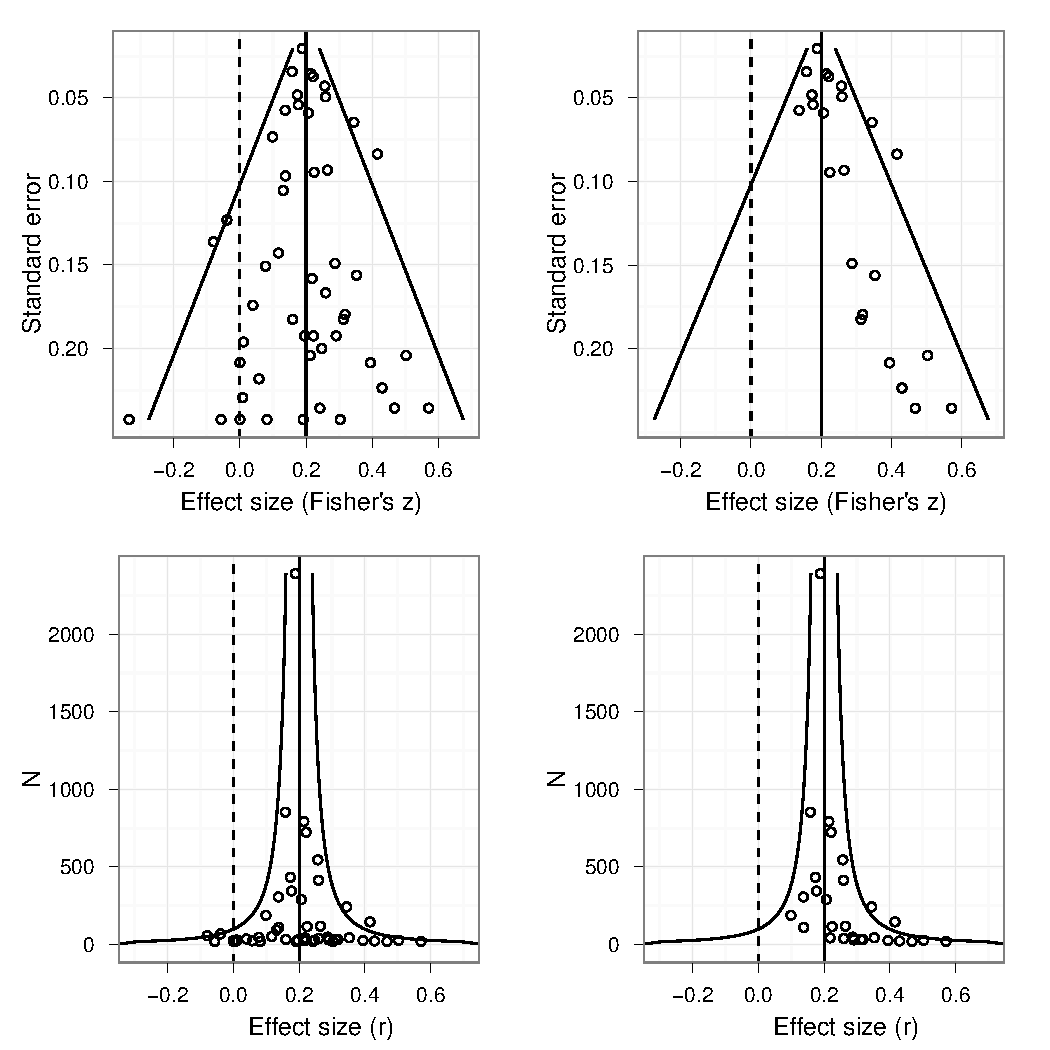
\includegraphics[width=0.68\linewidth]{f_02_FunnelCorrTotal}
  \end{center}
  \citep[Quelle: n.s: $p>0.10$][666]{weis_identification_2011}
\end{frame}



 \begin{frame}
   \frametitle{Trim and Fill}
   \begin{itemize}
   \item Imputationsansatz: Neben den beobachteten $k$ Studien existieren noch
     $k_0$ Studien, die aufgrund des \emph{Publication Bias} nicht ermittelt werden
     konnten.
   \item Aufgabe des Algorithmus ist, die Anzahl und die Ausprägungen dieser
     $k_0$ Studien zu schätzen.
   \item Ein Funnelplot mit den beobachteten und den geschätzten Effektstärken
     vermittelt einen guten Eindruck einer symmetrischen
     Effektstärkenverteilung.
   \item Gleichwohl belegt die Existenz von $k_0$ Studien nicht einen
     \emph{Publication Bias}, es wird erst einmal nur auf eine Asymmetrie der
     Effektstärkenverteilung in Abhängkeit von deren Reliabilität hingewiesen.
   \end{itemize}
 \end{frame}



 \begin{frame}
   \frametitle{Beispiel für Trim and Fill}
   %%
   \begin{center}
     \includegraphics[width=0.92\textwidth]{f_04_FunnelCorrTrimFill}
   \end{center}
   \citep[Quelle: ][671]{weis_identification_2011}.
 \end{frame}



 \begin{frame}
   \frametitle{Korrelationsverfahren}
   Berechnung der Rangkorrelation (Kendall's Rang-Korrelation) zwischen
   (z-standardisierten) Effektstärken und Fehlervarianzen. Ein
   nicht-signifikanter Test deutet auf eine \emph{unverzerrte} Stichprobe hin.
 \end{frame}


  \begin{frame}
   \frametitle{Eggers lineares Regressionsmodell}

   \begin{itemize}
   \item Es wird ein bivariates lineares Regressionsmodell geschätzt.
   \item Als abhängige Variable wird die am Standardfehler normierte
     Effektstärke ($\frac{T_j}{SE_j}$) benutzt.
   \item Das unabhängige Merkmal ist der inverse Standardfehler
     ($\frac{1}{SE_j}$) (\emph{precision}).
   \item Liegt \emph{keine} Verzerrung vor, sollte die Regressionsgerade durch
     den Ursprung laufen ($H_0: \beta_0 = 0$). Warum?:
     \begin{itemize}
     \item $\frac{1}{SE_j}$ nähert sich für kleine Studien 0 (x-Achse).
     \item $\frac{T_j}{SE_j}$ näher sich für kleine Studien auch 0 (y-Achse).
     \end{itemize}

   \end{itemize}
   \citep[Quellen: ][]{egger_bias_1997, sterne_regression_2005}
 \end{frame}


 \begin{frame}[plain, shrink = 5]
   \frametitle{Beispiel für "`Egger's linear regression method"'}
   %%
  \begin{center}
    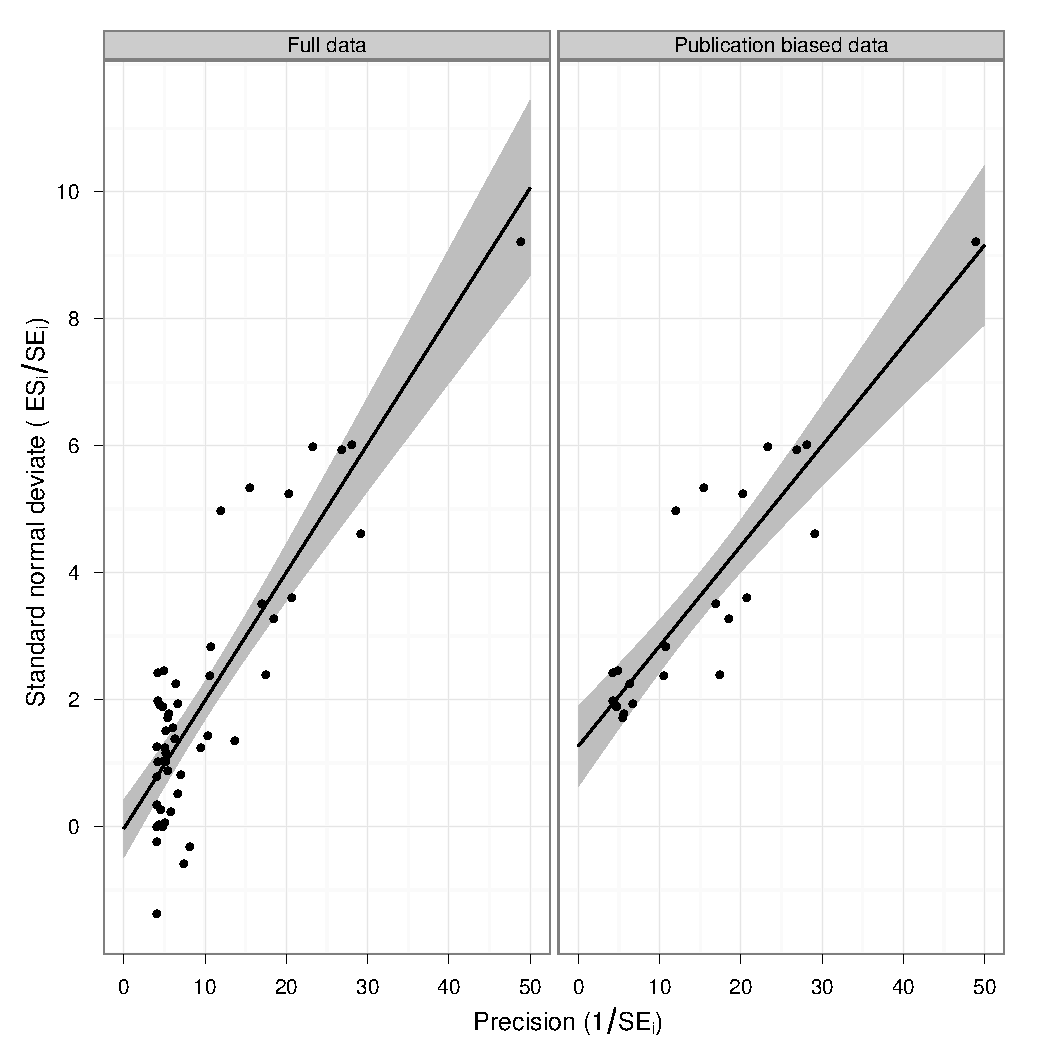
\includegraphics[width=0.91\textheight]{f_03_CompRegPlots}
  \end{center}
  \citep[Quelle: basiert auf simulierten Daten, siehe Folie \pageref{slide:funnel-sim-data};][669]{weis_identification_2011}.
 \end{frame}


\section{Reporting Standards}


\begin{frame}[allowframebreaks]\frametitle{Übersicht Reporting Standards}

  \begin{footnotesize}
    \begin{itemize}
    \item \fullcite{apa_reporting_2008}
    \item \fullcite{stroup_meta-analysis_2000}
    \item \fullcite{liberati_prisma_2009}
    \item \fullcite{riley_meta-analysis_2010}
    \item \fullcite{maer_network_maer_2012}
    \end{itemize}

    (Alle Standards finden sich als PDF-Dateien auch im Verzeichnis
    \texttt{ref/})
  \end{footnotesize}
\end{frame}


\begin{frame}[allowframebreaks]\frametitle{MAER-Net Reporting Standards}
  Quelle: \url{http://www.hendrix.edu/MAER-Network/post.aspx?id=62556&blogid=51160}
  \\ \vspace{1ex}
  MAER-Net (Meta-Analysis of Economics Research (MAER) Network) recommends that
  all meta-analyses in economics should comply with the following reporting
  protocols.

\begin{itemize}
\item Research Questions and Effect Size
  \begin{itemize}
  \item A clear statement of the specific economic theories, hypotheses, or
    effects studied.
  \item A precise definition of how effects are measured (the ‘effect size’),
    accompanied by any relevant formulas.
  \item An explicit description about how measured effects are comparable,
    including any methods used to standardize or convert them to a common
    metric.
  \end{itemize}
\item Research Literature, Searching, Compilation and Coding
  \begin{itemize}
  \item A  full report of how the research literature was searched.  This report should include:
    \begin{itemize}
    \item the exact databases or other sources used;
    \item the precise combination of keywords employed; and
    \item the date that the search was completed.
    \end{itemize}
  \item A full disclosure of the rules for study (or effect size)
    inclusion/exclusion.  It is also useful to provide a list of all studies
    included and a description of why others were excluded.
  \item A statement addressing who searched, read, and coded the research
    literature. Two or more reviewers should code the relevant research.
  \item A complete list of the information coded for each study or estimate. At
    a minimum, we recommend that reviewers code:
    \begin{itemize}
    \item the estimated effect size;
    \item its standard error, when feasible, and the degrees of freedom (or sample size);
    \item variables that distinguish which type of econometric model, methods and techniques were employed;
    \item dummy (i.e., 0/1) variables for the omission of theoretically relevant
      variables in the research study investigated;
    \item empirical setting (e.g., region, market, industry);
    \item data types (panel, cross-sectional, time series, . . . );
    \item year of the data used and/or publication year;
    \item type of publication (journal, working paper, book chapter, etc.); and
    \item the primary study, publication and/or dataset from which an observation is drawn.
    \end{itemize}
  \end{itemize}
\item MRA Modeling Issues
  \begin{itemize}
  \item A table of descriptive statistics of the variables that are coded (means
    and standard deviations) and graph(s) displaying the effect sizes (e.g.,
    funnel graphs, forest plots, bar charts).
  \item A fully reported multiple MRA, along with the exact strategy used to
    simplify it (e.g., general-to-specific, Bayesian).
  \item An investigation of publication, selection, and misspecification biases.
    When suspected, these should be controlled for in subsequent MRA models.
  \item Methods to accommodate heteroscedasticity and within-study dependence.
  \item Results from MRA model specification tests, robustness checks, or sensitivity analyses.
  \end{itemize}

\end{itemize}

With one possible exception, MAER-Net has come to a clear consensus about these
reporting guidelines.  The requirement to have two reviewers code all the
relevant research has received the most comment and discussion.  As economists,
we all are acutely aware of the trade-off between the improved quality that the
second coder will likely add (through catching mistakes and resolving
ambiguities) and the increased cost (in weeks of highly skilled professional
labour). We understand that the highest standards of scientific rigor demand at
least two highly-knowledgeable researchers code the relevant research base.
Nonetheless, MAER-Net does not wish to prohibit Ph.D. students and researchers
at resource-challenged institutions from employing this important tool
to understand their areas of research.  To finesse these opposing concerns, the
above statement is sufficiently broad to encompass a second reviewer randomly
checking a substantial proportion of the research literature if their coding
protocol is stated explicitly and justified.


\end{frame}




\section{Ein Ausblick auf Meta-Analysen mit Individualdaten}

\begin{frame}\frametitle{Was ist eine IPD Meta-Analyse?}

  \begin{quotation}
    \enquote{As with any meta-analysis, an individual participant data meta-analysis aims
    to summarise the evidence on a particular clinical question from multiple
    related studies, such as whether a treatment is effective. The statistical
    implementation of an individual participant data meta-analysis crucially
    \alert{must preserve the clustering of patients within studies}; it is inappropriate
    to simply analyse individual participant data as if they all came from a
    single study. Clusters can be retained during analysis by using a two step
    or a one step approach.}
  \end{quotation}

  \citep[Quelle: ][1]{riley_meta-analysis_2010}

\end{frame}


\begin{frame}\frametitle{APD und IPD Meta-Analysen}
  \begin{itemize}
  \item Meta-Analysen auf der Grundlage von \emph{Aggregate Person Data} (APD)
  \item Meta-Analysen auf der Grundlage von \emph{Individual Person/Participant/Patient Data}
    \begin{itemize}
    \item Einstufige Ansätze: (Mehrebenen-)Regressionsmodelle auf der Grundlage eines gepoolten Datensatzes
    \item Zweistufige Ansätze: pro Datensatz eine Effekstärke berechnen und anschließend eine APD Meta-Analyse durchführen
    \end{itemize}
  \item Meta-Analysen, die sowohl APD und IPD verwenden.
  \end{itemize}
\end{frame}



\begin{frame}\frametitle{Vorteile von IPD Meta-Analysen}
  %%
  \begin{footnotesize}
    \begin{itemize}
    \item Erhöhte Auswahl angemessener Analyseverfahren, etwa für die Analyse
      von nicht-experimentellen Daten (multivariate Auswertungstechniken).
    \item Zentrale Merkmale lassen sich vereinheitlichen, erhöht die
      Vergleichbarkeit der Konstrukte.
    \item Bei zweistufigem Vorgehen keine Probleme mit fehlenden ES-Angaben.
    \item Es lassen sich zusätzliche Hypothesen untersuchen, insbesondere
      solche, die mit individuellen Charakteristika zusammenhängen.
    \item U.U. größere statistische \emph{power}, um Interaktionen zwischen
      Studienmerkmalen und ES zu finden.
    \item Schließlich besteht bei der Verwendung von Aggregatdaten immer die
      Gefahr eines ökologischen Fehlschlusses.
    \end{itemize}
    \citep[Quelle: ][252]{weis_potentiale_2008, pigott_advances_2012}
  \end{footnotesize}
\end{frame}


\begin{frame}\frametitle{Nachteile von IPD Meta-Analysen}
  \begin{itemize}
  \item Hoher Kosten- und Zeitaufwand (vor allem Medizin, teilw. Kooperationen von mehreren dutzend Partnern).
  \item Nicht immer sind \emph{alle} vorhandenen Datensätze auch verfügbar.
  \item Große Datensätze und anspruchsvolle Analyseverfahren können Desktop-PCs überfordern.
  \end{itemize}
\end{frame}


\begin{frame}\frametitle{Eigene Erfahrungen mit einer IPD Meta-Analysen}
  \begin{itemize}
  \item Forschungsprojekt: "`How employment status affects partnership stability: A meta-analysis using longitudinal individual person data"'
  \item 16 Längsschnittdatensätze aufbereiten
  \item Gepoolter Datensatz wird (im "`person-period format"') mehrere Millionen Zeilen umfassen
  \item (Sehr/Zu?) Komplexe Dokumentation zur Datenaufbereitung (diskrete EHA)
  \item Offene Probleme:
    \begin{itemize}
    \item Umgang mit Gewichten
    \item Sehr aufwändige Datenaufbereitung (techn. Infrastruktur, Organisation der Skripte, Dokumentation, \ldots)
    \end{itemize}
  \item \ldots
  \end{itemize}
\end{frame}


\begin{frame}[allowframebreaks]\frametitle{Literatur zu IPD Meta-Analysen}
  \begin{footnotesize}
    \begin{itemize}
    \item \fullcite{stewart_ipd_2002}
    \item \fullcite{simmonds_meta-analysis_2005}
    \item \fullcite{riley_meta-analysis_2007}
    \item \fullcite{sutton_meta-analysis_2008}\footnote{Mit einem Bayesianischen Modell Kombination von IPD und
        APD Meta-Analyse.}
    \item \fullcite{cooper_relative_2009}
    \item \fullcite{curran_integrative_2009}
    \item \fullcite{riley_meta-analysis_2010}
    \item \fullcite{pigott_advances_2012} (insbes. Kapitel 8)
    \end{itemize}
  \end{footnotesize}
\end{frame}


\section{Literatur}

\begin{frame}[allowframebreaks]\frametitle{Literaturempfehlungen und weitere Informationsquellen}

  \begin{footnotesize}
    \begin{itemize}
    \item Literatur
      \begin{itemize}
      \item \fullcite{borenstein_introduction_2009}
      \item \fullcite{lipsey_practical_2001}
      \item \fullcite{cooper_research_2010}
      \item \fullcite{petticrew_systematic_2006}
      \item \fullcite{cooper_handbook_2009}
      \end{itemize}
    \item Zeitschriften
      \begin{itemize}
      \item Research Synthesis Methods
        <\url{http://onlinelibrary.wiley.com/journal/10.1002/\%28ISSN\%291759-2887}>
      \item Statistics in Medicine
        <\url{http://onlinelibrary.wiley.com/journal/10.1002/\%28ISSN\%291097-0258}>
      \item Systematic Reviews <\url{http://www.systematicreviewsjournal.com/}>
      \end{itemize}
    \item Organisationen
      \begin{itemize}
      \item The Cochrane Collaboration <\url{http://www.cochrane.org/}>
      \item The Campbell Collaboration
        <\url{http://www.campbellcollaboration.org/}>
      \end{itemize}
    \end{itemize}
  \end{footnotesize}
\end{frame}

\renewcommand{\bibfont}{\normalfont\tiny}
\begin{frame}[allowframebreaks, plain]\frametitle{Literatur}
\printbibliography
\end{frame}




%%% Local Variables:
%%% TeX-master: "ps2012gesis-ma-workshop.tex"
%%% End:
